% To je predloga za poročila o domačih nalogah pri predmetih, katerih
% nosilec je Blaž Zupan. Seveda lahko tudi dodaš kakšen nov, zanimiv
% in uporaben element, ki ga v tej predlogi (še) ni. Več o LaTeX-u izveš na
% spletu, na primer na http://tobi.oetiker.ch/lshort/lshort.pdf.
%
% To predlogo lahko spremeniš v PDF dokument s pomočjo programa
% pdflatex, ki je del standardne instalacije LaTeX programov.

\documentclass[a4paper,11pt]{article}
\usepackage{a4wide}
\usepackage{fullpage}
\usepackage[utf8x]{inputenc}
\usepackage[slovene]{babel}
\selectlanguage{slovene}
\usepackage[toc,page]{appendix}
\usepackage[pdftex]{graphicx} % za slike
\usepackage{setspace}
\usepackage{color}
\definecolor{light-gray}{gray}{0.95}
\usepackage{listings} % za vključevanje kode
\usepackage{hyperref}
\renewcommand{\baselinestretch}{1.2} % za boljšo berljivost večji razmak
\renewcommand{\appendixpagename}{Priloge}

\lstset{ % nastavitve za izpis kode, sem lahko tudi kaj dodaš/spremeniš
language=Python,
basicstyle=\footnotesize,
basicstyle=\ttfamily\footnotesize\setstretch{1},
backgroundcolor=\color{light-gray},
}

\title{Logisti\v{c}na regresija}
\author{Gregor Majcen (63070199)}
\date{\today}

\begin{document}

\maketitle

\section{Uvod}
Cilj sedme doma"ce naloge je implementacija logisti"cne regresije z regularizacijo. Kaj to"cno to pomeni, je podrobneje opisano v naslednjih poglavjih. Uspe"snost na"se implementacije je potrebno dokazati na realnih podatkih (iz prej"snje naloge) in sicer s 5-kratnim pre"cnim preverjanjem. Da doka"zemo, kako mo"cno je regularizacija pomembna bomo to tudi testirali in primerjali rezultate. 

\section{Podatki in opis problemske domene}
Podatki, ki jih preiskujemo so s podro"cja kemoinformatike. Podatke so bolj podrobno opisani ze v prej"snji nalogi, ampak izpostavimo najpomembnej"se. Imamo 1776 atributov, 3751 primerov in en binaren razred. Kot zelo pomemben podatek je, da so atributi normalizirani. V peti doma"ci nalogi smo ugotovili, da pomaga pri hitrosti iskanju minimuma linearne regresije. Za bolj to"cno ra"cunanje smo dodali se dodatnih n*1776 atributov, ki so vsi prej"snji $attr^2$, $attr^3$, \ldots, $attr^n$. S tem smo simulirali vi"sjo stopnjo polinoma.  Zaradi prevelikega prileganja podatkov je tu potrebna "se regularizacija.

\section{Metoda}
Logisti"cna regresija je metoda za klasifikacijo diskretnih problemov. Je zelo podobna linearni regresiji, ki smo jo implementirali v eni izmed prej"snjih nalog. Edina razlika je v na"si hipotezi h. 

Pri linearni regresiji je $h_\theta(x) = \theta^Tx$, kar pa tu ne pride ve"c v po"stev, saj ni razloga, zakaj bi hoteli imeti ciljne vrednosti ve"cje od 1 ali manj"se od 0. To popravimo s tako imenovano \textit{sigmoidno funkcijo} $g(z) = {1\over{1+e^{-z}}}$. Sigmoidna funkcija je vse kar potrebujemo: je monotono nara"s"cujo"ca, zavzema vrednosti $(0,1)$ in ima zelo lep odvod: $g'(z) = g(z)(1-g(z))$.

Na"sa nova funkcija za hipotezo je torej $h_\theta(x) = g(\theta^Tx) = {1\over{1+e^{-\theta^Tx}}}$

Ker je sedaj razred binaren, lahko tudi \textit{verjetje} (ang. likelihood) zelo poenostavimo. Kot vemo "ze od prej"snji"c, mora biti verjetje "cimve"cje. Za la"zje ra"cunanje raje vzamemo logaritem verjetja:
\[l(\theta) = \sum_{i=1}^my^{(i)}*log(h(x^{(i)})) + (1-y^{(i)})*log(1-h(x^{(i)}))\]
in njegov odvod 
\[{\partial\over{\partial\theta_j}}l(\theta) = (y-h_\theta(x))x_j\]
Cenovna funkcija, ki jo potrebujemo za na"s algoritem je $-l(\theta)$ in jo je potrebno minimizirati. Posledi"cno se tudi pri odvodu doda negativen predznak. $-{\partial\over{\partial\theta_j}}l(\theta)$ je torej na"sa gradientna funkcija. S pomo"cjo "ze znanega in kar hitrega algoritma L-BFGS poi"s"cemo minimum cenovne funkcije in kot rezultat dobimo optimalne $\theta$.

Zaradi simuliranja vi"sje stopnje polinoma se podatki preve"c prilagajajo. Zato je potrebna regularizacija. Na"si cenovni funkciji pri"stejemo "se $\lambda * \sum_{i=1}^n\theta_i^2$, kjer je $\lambda$ poljuben parameter. Posledi"cno je potrebno spremeniti tudi gradientno funkcijo. Tu pa pri"stejemo $\lambda * \sum_{i=1}^n2*\theta_i$. Na sliki~\ref{slika1} je lepo razvidno, kako se funkcije prilagajajo.

\begin{figure}[h!]
\begin{center}
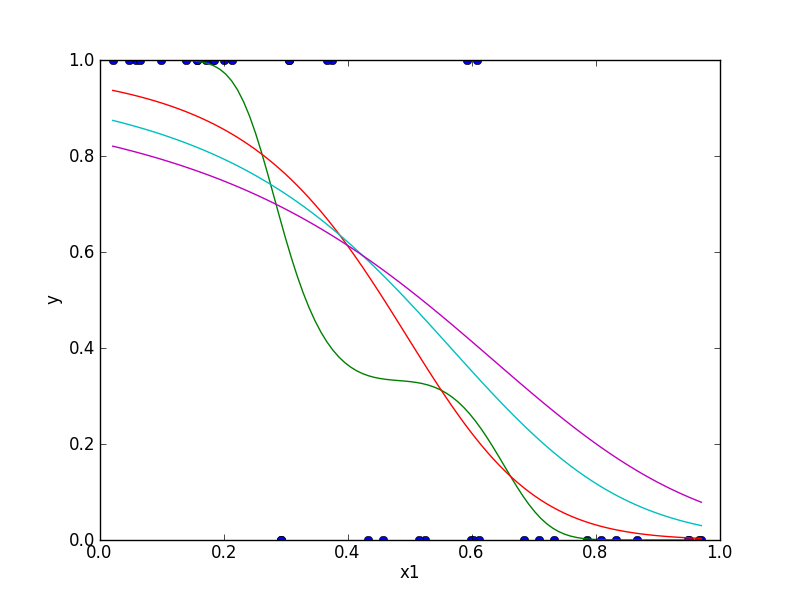
\includegraphics[scale=0.6]{slika1}
\caption{Sigmoidna funkcija pri razli"cnih vrednosti $\lambda$}
\label{slika1}
\end{center}
\end{figure}

\pagebreak

\section{Rezultati}
Logisti"cno regresijo sem testiral s 5-kratnim pre"cnim preverjanjem in izra"cunal logLoss oceno.
\begin{table}[h]
\centering
\begin{tabular}{l|l|l}
Stopnja polinoma & $\lambda$ & logLoss\\
\hline
2 & 0 & 2.62 \\
1 & 0.01 & 0.50 \\
1 & 0.005 & 0.52 \\
2 & 0.01 & 0.51 \\
2 & 0.001 & 0.58 \\
3 & 0.01 & 0.52 \\
3 & 0.001 & 0.62 \\
\end{tabular}
\caption{tabela rezultatov}
\label{t:rez}
\end{table}

V tabeli~\ref{t:rez} je tudi lepo razvidno, da brez regularizacije enostavno ne gre. S pomo"cno posku"sanj sem dobil najbolj"se rezultate pri $\lambda = 0.01$ in originalnih podatkih. V tabeli so prikazani le pomembnej"si rezultati.

\section{Izjava o izdelavi domače naloge}
Domačo nalogo in pripadajoče programe sem izdelal sam.

\end{document}
